\documentclass[12pt,english,pdf,dvipsnames,handout]{beamer}
\usepackage{fontspec}
\setsansfont[Mapping=tex-text]{Fira Sans}
\setcounter{secnumdepth}{4}
\setcounter{tocdepth}{4}
\usepackage[normalem]{ulem}
\usepackage[T1]{fontenc}
\usepackage{dcolumn}
\usepackage{booktabs}
\usepackage{setspace}
\makeatletter
\usetheme[progressbar=frametitle,block=fill]{metropolis}
\metroset{background=dark}
\usepackage{mathpazo}
\usepackage{xcolor}
\definecolor{title}{RGB}{255,98,0}
\usepackage{tikz, tikz-cd}
\usetikzlibrary{shapes,backgrounds,trees,decorations.pathreplacing}
\usepackage[labelformat=empty]{caption}
\usepackage{pgfplots}
\pgfplotsset{compat=1.15}
\usepgfplotslibrary{fillbetween}
\usepackage{pgfplotstable}
\usepackage[sectionbib]{apacite}
\renewcommand{\bibliographytypesize}{\footnotesize}
\usepackage{amsmath}
\usepackage{polyglossia}
\setdefaultlanguage[variant=american]{english}
\usepackage{multirow}
\usepackage{subcaption}
\usepackage{wrapfig}
\usepackage{hyperref}
\hypersetup{pdfauthor={Constantin Manuel Bosancianu},
pdftitle={Data Visualization with R},
pdfsubject={Slides for SPP CEU course},
pdfkeywords={Budapest, CEU, SPP, 2021, visualization}}
% Defines a checkmark
\def\checkmark{\tikz\fill[scale=0.4, color=title](0,.35) -- (.25,0) -- (1,.7) -- (.25,.15) -- cycle;}
\setbeamertemplate{itemize items}{\checkmark}

\title{\textsc{Data Visualization with R}}
\subtitle{Principles and Practice}
\author{Constantin Manuel Bosancianu}
\institute{Wissenschaftszentrum Berlin \\ \textit{Institutions and Political Inequality} \\\href{mailto:bosancianu@icloud.com}{bosancianu@icloud.com}}
\date{May 5, 2021}
\begin{document}
\maketitle
% PREAMBLE %

\section{Preamble}

\begin{frame}{Plan for today}
  Things to speak about:

  \begin{itemize}
  \item The importance of data visualization;
  \item Basics of \textit{good} data visualization;
  \item ``The \textit{good}, the \textit{bad}, and the \textit{ugly}'' when it comes to data visualization---examples.
  \end{itemize}

  \bigskip
The rest of the course is hands-on, using \texttt{R} and \texttt{ggplot2}.
  
\end{frame}


\section{Introduction}

\begin{frame}{Importance}
There is more data than ever waiting to be analyzed, mined for patterns, summarized, or linked to other data.\bigskip

\pause

We also observe a phenomenal level of growth in individual-level data: Internet, GPS-enabled smartphones, e-scooters, smartwatches, fitness trackers, automated sensors, smart speakers etc.
  
\end{frame}


\begin{frame}{Importance}

Presenting such information in an accurate and intuitive way for the purpose of highlighting causal connections will be crucial for our ability to make adequate choices in a democracy.
  
\end{frame}




\section{Principles}

\begin{frame}{Data visualization (DV)}
  At the confluence between statistics and design, dealing with the search for the most effective and graphically intuitive way of making an argument on the basis of data.\bigskip

  In 2000, an estimated 900 billion ($9*10^{11}$) to 2 trillion ($2*10^{12}$) graphs were generated every year \cite{Tufte2001}.
  
\end{frame}


\begin{frame}{Goals of DV}
  Multiple:

  \begin{itemize}
  \item Making an argument;
  \pause
  \item Minimizing any distractions from the central argument;
  \pause
  \item Ensuring the integrity of the argument;
  \end{itemize}
\bigskip
\pause
``Making a presentation is a moral act as well as an intellectual activity.'' \cite[p.~141]{Tufte2006}
  
\end{frame}


\begin{frame}{Simple, yet effective}

\begin{figure}
	\centering
	\includegraphics[scale=0.4]{../04-graphs/27_GOP_Dem_Bartels}
	\caption{Economic performance under US presidents \cite{Bartels2008a}}
\end{figure}

\end{frame}


\begin{frame}{Goals of DV}
  Two more:

  \begin{itemize}
  \item Summarizing a lot of information in a reduced space;
  \pause
  \item Encouraging comparison.
  \end{itemize}
  
\end{frame}


\begin{frame}{Principles of DV \cite<adapted from>[]{Tufte2001}}

  \begin{itemize}
  \item The overarching purpose is to show the data;\bigskip
  \pause
  \item Minimize the data-ink ratio, as much as possible;\bigskip
  \pause
  \item Erase non-data-ink, as much as possible;\bigskip
  \pause
  \item Minimize redundant data-ink, as much as possible;\bigskip
  \pause
  \item Revise and edit;\bigskip
  \pause
  \item Mobilize every graphical element needed.
  \end{itemize}
  
\end{frame}


\begin{frame}{Keeping it simple}

\begin{figure}
	\centering
	\includegraphics[scale=0.40]{../04-graphs/29_Cluttered_boxplot}
	\caption{Should be as simple as it needs to be, but not more}
\end{figure}

\end{frame}


\begin{frame}{Keeping it simple}

\begin{figure}
	\centering
	\includegraphics[scale=0.75]{../04-graphs/30_Clean_boxplot}
\end{figure}

\end{frame}



\begin{frame}{ACCENT principles \cite<from>[]{Burn1993}}
  \textcolor{title}{A}pprehension: ability to correctly perceive relations among variables.\bigskip

  \pause

  \textcolor{title}{C}larity: Ability to visually distinguish all the elements of a graph.\bigskip

  \pause

  \textcolor{title}{C}onsistency: Ability to interpret a graph based on similarity to previous graphs.
\end{frame}


\begin{frame}{ACCENT principles}
  \textcolor{title}{E}fficiency: Ability to portray a possibly complex relation in as simple a way as possible.\bigskip

  \pause

  \textcolor{title}{N}ecessity: The need for the graph, and the graphical elements.\bigskip

  \pause

  \textcolor{title}{T}ruthfulness: Ability to determine the true value represented by any graphical element by its magnitude relative to the implicit or explicit scale.
\end{frame}

  

\section{Good examples}

\subsection{Minard's graph}
\begin{frame}{Napoleon's 1812--1813 campaign}

\begin{figure}
  \centering
  \includegraphics[scale=0.15]{../04-graphs/01_Minard_map}
  \caption{Multiple dimensions on a 2-dimensional map}
\end{figure}

Temperature, deaths, movement, advance/retreat.

\end{frame}

\begin{frame}{Multiple ways of presenting}

\begin{tabular}{cl}  
       \begin{tabular}{c}
         \includegraphics[scale=0.275]{../04-graphs/02_Minard_redesign_Boykin}
       \end{tabular}
    & \begin{tabular}{l}
        \parbox{0.4\linewidth}{Map matters less than number of deaths, advance/retreat, and temperature.\bigskip

        Emphasis on dismal rate of survival.\bigskip

        Temperature matters more in winter.}
      \end{tabular}  \\
\end{tabular}

\end{frame}


\begin{frame}{Focus on a single aspect}

\begin{tabular}{cl}  
       \begin{tabular}{c}
         \includegraphics[scale=0.6]{../04-graphs/03_Minard_single_focus}
       \end{tabular}
    & \begin{tabular}{l}
        \parbox{0.4\linewidth}{A simple point shouldn't require a complex graph.}
      \end{tabular}  \\
\end{tabular}
  
\end{frame}



\subsection{Relative billions}
\begin{frame}{Getting a sense of large numbers}

\begin{figure}
  \centering
  \includegraphics[scale=0.425]{../04-graphs/04_Billion_pound_gram}
\end{figure}

\end{frame}


\begin{frame}{(not really intended for accurate comparisons\dots}

\begin{figure}
  \centering
  \includegraphics[scale=0.35]{../04-graphs/05_Billion_dollar_gram_1}
\end{figure}

\end{frame}


\begin{frame}{\dots but rather for relative dimensions)}

\begin{figure}
  \centering
  \includegraphics[scale=0.35]{../04-graphs/06_Billion_dollar_gram_2}
\end{figure}

\end{frame}


\begin{frame}{Putting it into perspective}

\begin{tabular}{cl}  
       \begin{tabular}{c}
       \includegraphics[scale=0.35]{../04-graphs/07_Billion_dollar_gram_3}
       \end{tabular}
    & \begin{tabular}{l}
        \parbox{0.4\linewidth}{Cost of crisis over 2008--2016 estimated at 4.6 trillion USD.\bigskip

        \tiny{\url{https://hbr.org/2018/09/the-social-and-political-costs-of-the-financial-crisis-10-years-later}}}
      \end{tabular}  \\
\end{tabular}

\end{frame}


\subsection{Visualizing association}

\begin{frame}{Ontario welfare benefits}

\begin{figure}
  \centering
  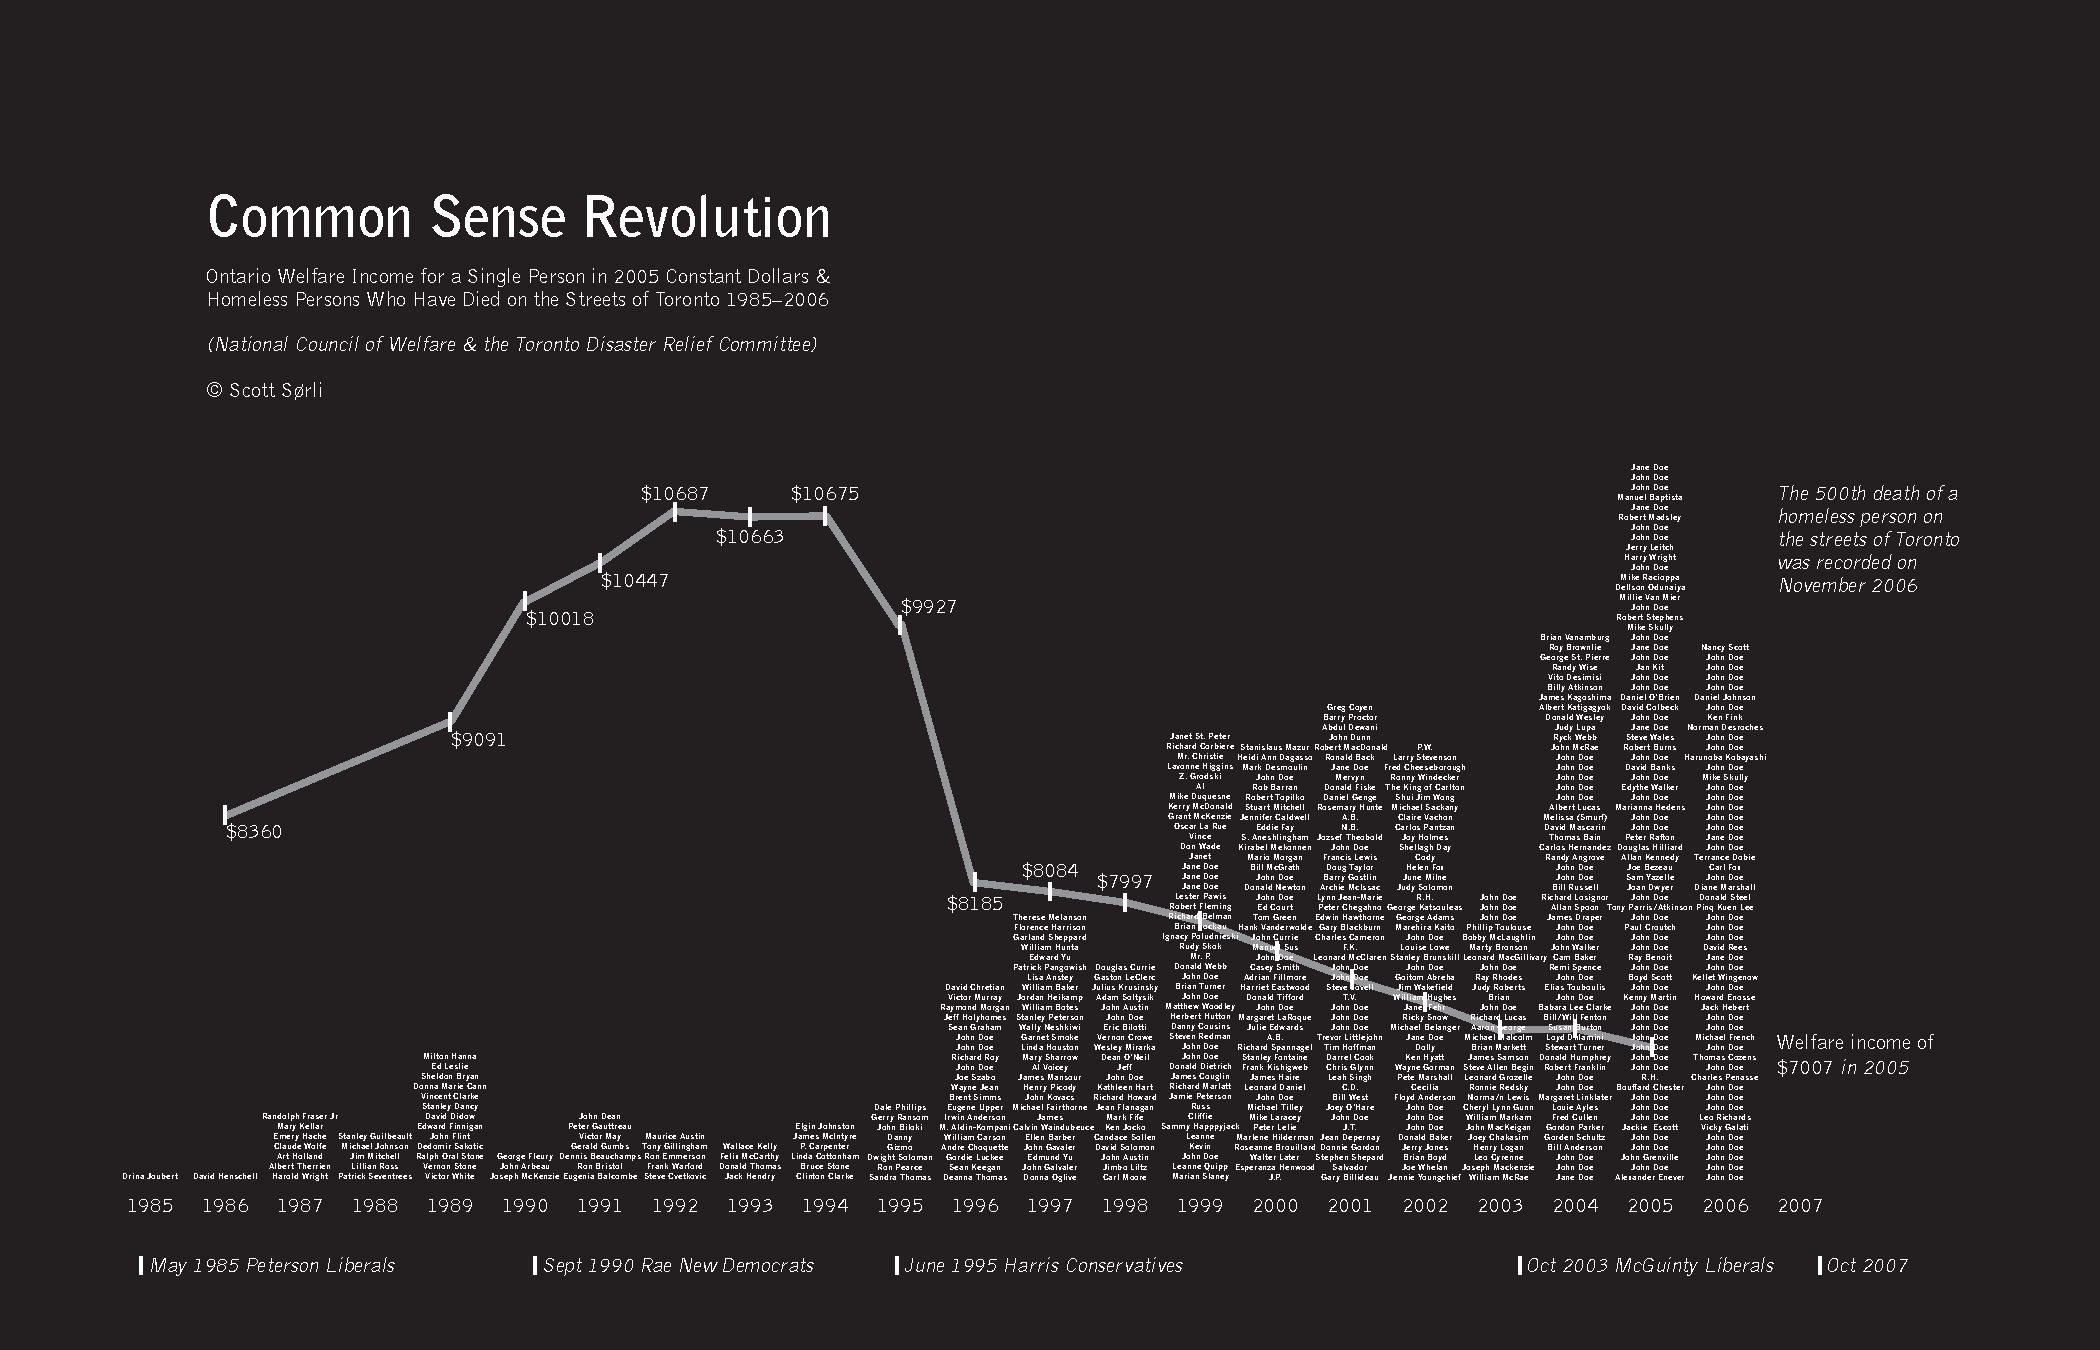
\includegraphics[scale=0.30]{../04-graphs/09_Ontario_welfare}
\end{figure}

\end{frame}




\section{Bad examples}

\begin{frame}{Violations of basic rules \cite{Tufte2001}}

\begin{enumerate}
	\item Showing more dimensions than there are in the data
	\pause
	\item Showing surfaces which are disconnected from the underlying quantities
	\pause
	\item Varying the design even though the data isn't varying
	\pause
	\item Failing to adjust for inflation, population change etc. in time-series data
	\pause
	\item Failing to provide adequate context for the data
	\pause
	\item Failing to put proper labels on axes
\end{enumerate}


\end{frame}


\subsection{Chartjunk}
\begin{frame}{Chartjunk}

\begin{figure}
  \centering
  \includegraphics[scale=0.4]{../04-graphs/10_Monster_costs}
  \caption{Unnecessary features galore (keep in mind, though: they might be easier to recall)}
\end{figure}

\end{frame}


\begin{frame}{Chartjunk}

\begin{figure}
  \centering
  \includegraphics[scale=0.4]{../04-graphs/11_Diamonds}
  \caption{Unnecessary features (and sexism) galore (these are aesthetic violations, following \citeNP{Healy2018})}
\end{figure}

\end{frame}


\begin{frame}{Chartjunk}
	
	\begin{figure}
		\centering
		\includegraphics[scale=0.25]{../04-graphs/36_WEF_women_leadership}
		\caption{Unnecessary features, and poor choice of display}
	\end{figure}
	
\end{frame}


\subsection{Misleading graphs}

\begin{frame}{Toying with perception}

\begin{figure}
  \centering
  \includegraphics[scale=0.45]{../04-graphs/12_Fuel_economy}
  \caption{Supports the point of radical government overreach}
\end{figure}

\end{frame}


\begin{frame}{Toying with perception}

\begin{tabular}{cl}  
       \begin{tabular}{c}
       \includegraphics[scale=0.45]{../04-graphs/13_College_rank}
       \end{tabular}
    & \begin{tabular}{l}
        \parbox{0.4\linewidth}{3 things seem wrong here to me.}
      \end{tabular}  \\
\end{tabular}

\end{frame}


\begin{frame}{Toying with perception}

\begin{figure}
	\centering
	\includegraphics[scale=0.65]{../04-graphs/22_Venezuela_elections}
\end{figure}

\end{frame}


\begin{frame}{Toying with perception}

\begin{figure}
	\centering
	\includegraphics[scale=0.5]{../04-graphs/23_NSW_health}
\end{figure}

\end{frame}


\begin{frame}{Toying with perception}
	
	\begin{figure}
		\centering
		\includegraphics[scale=0.5]{../04-graphs/32_Trump_misleading_tweet}
	\end{figure}
	
\end{frame}


\begin{frame}{Toying with perception}
	
	\begin{figure}
		\centering
		\includegraphics[scale=0.11]{../04-graphs/33_Trump_plot_enlarged}
	\end{figure}
	
\end{frame}


\begin{frame}{Toying with perception}
	
	\begin{figure}
		\centering
		\includegraphics[scale=0.24]{../04-graphs/40_Mercurio_Chile_statistics}
	\end{figure}
	
\end{frame}


\begin{frame}{``Perfect storm'' of a bad plot}

\begin{figure}
	\centering
	\includegraphics[scale=0.5]{../04-graphs/24_Fox_unemployment}
	\caption{At least 3 things are wrong here}
\end{figure}

\end{frame}



\begin{frame}{Trimming a trend}

\begin{figure}
  \centering
  \includegraphics[scale=0.35]{../04-graphs/14_Traffic_deaths_1}
  \includegraphics[scale=0.35]{../04-graphs/15_Traffic_deaths_2}
\end{figure}

\end{frame}


\subsection{Poor statistics}
\begin{frame}{Statistics misreported}

\begin{figure}
	\centering
	\includegraphics[scale=0.45]{../04-graphs/16_Fox_piechart}
\end{figure}

\end{frame}


\begin{frame}{Statistics misreported}

\begin{figure}
	\centering
	\includegraphics[scale=0.45]{../04-graphs/17_CBS_piechart}
\end{figure}

\end{frame}


\begin{frame}{Statistics misreported}

\begin{tabular}{cl}  
	\begin{tabular}{c}
    \includegraphics[scale=0.45]{../04-graphs/18_Happiness_plateau}
	\end{tabular}
	& \begin{tabular}{l}
	\parbox{0.35\linewidth}{The puzzle is based on the assumption that the relationship should be linear.}
	\end{tabular}  \\
\end{tabular}

\end{frame}

\begin{frame}{Statistics misreported}
	
	\begin{tabular}{cl}  
		\begin{tabular}{c}
			\includegraphics[scale=0.15]{../04-graphs/41_Georgia_covid_t}
		\end{tabular}
		& \begin{tabular}{c}
			\includegraphics[scale=0.135]{../04-graphs/42_Georgia_covid_t_plus_15days}
		\end{tabular}  \\
	\end{tabular}
	
\end{frame}


\begin{frame}{Bad data}

\begin{figure}
	\centering
	\includegraphics[scale=0.3]{../04-graphs/25_Democracy_danger}
\end{figure}

Difference between those who respond ``10'' and the rest.

\end{frame}



\begin{frame}{Better data}

\begin{figure}
	\centering
	\includegraphics[scale=0.115]{../04-graphs/26_Democracy_safe}
\end{figure}

Only 2 countries out of 5 keep their pattern; less concerning than before.
\end{frame}


\subsection{Poor graphs}
\begin{frame}{Poor choice of graphs}

\begin{figure}
	\centering
	\includegraphics[scale=0.38]{../04-graphs/19_Voltage_trend}
\end{figure}

\end{frame}


\begin{frame}{Poor choice of graphs}

\begin{figure}
	\centering
	\includegraphics[scale=0.55]{../04-graphs/20_Sotheby_Christie}
\end{figure}

\end{frame}


\begin{frame}{Poor choice of graphs}

\begin{figure}
	\centering
	\includegraphics[scale=0.55]{../04-graphs/21_OECD_health}
\end{figure}

\end{frame}


\begin{frame}{Improved display}

\begin{figure}
	\centering
	\includegraphics[scale=0.08]{../04-graphs/28_OECD_health_improved}
\end{figure}

\end{frame}




\section{Conclusion}

\begin{frame}{Conclusion}
Good data visualization involves thinking about the argument to be made, making choices among alternatives, and taking into consideration issues such as audience, parsimony, integrity.\bigskip

It will rarely result from canned routines and default options found in statistical packages.
\end{frame}


\begin{frame}{Conclusion}
With \texttt{ggplot2}, we wouldn't be able to fall prey to some bad practices, like creating chartjunk.\bigskip

However, there is still potential for other design issues: redundant information, large ink/data ratio, etc.
\end{frame}


% FRAME
\begin{frame}
\begin{center}
	\Huge Thank \textcolor{title}{you} for the kind attention!
\end{center}
\end{frame}

\begin{frame}[plain,c]
	\begin{center}
		\Huge References
	\end{center}
\end{frame}

% REFERENCES %

\begin{frame}[plain, allowframebreaks]
\renewcommand{\section}[2]{}
\bibliographystyle{apacite}
\bibliography{Works-cited}
\end{frame}

\end{document}